\subsection{Methodology}
We ran our local experiments on a Dell Precision T7500n Dual Processor desktop 
computer running 64-bit RHEL6 built on the 2.6.32 kernel for CentOS6. The 
machine housed a Dual Quad Core Intel\textsuperscript{\textregistered} 
Xeon\textsuperscript{\textregistered} E5620 2.40GHz Processor, 24GB of RAM, 
two 600GB 15K RPM hard drives and one 2TB hard drive.

In remote case, we ran \XXX{Jim, care to fill this up?}

\subsection{LSVD microbenchmarks}
First, we wanted to evaluate our LSVD implementation. Since LSVD exports interface very similar to a file, we can easily compare LSVD throughput to regular file throughput. These benchmarks were all run locally.

We evaluated LSVD using five benchmarks, which we ran in specific order:
\begin{enumerate}
\item \textbf{Sequential write} - Sequential write of 5GB random data to a new file/LSVD with 40KB buffers,
\item \textbf{Sequential read} - Sequential read of 5GB of previously created file with 40KB buffers,
\item \textbf{Random read} - Randomly read 128MB using 4KB buffers,
\item \textbf{Random write} - Randomly written 128MB using 4KB buffers,
\item \textbf{Sequential read 2} - Sequential read of 5GB of the file using 40KB buffers. However, this time we are also reading changes made by fourth benchmark.
\end{enumerate}

All read and write operations were performed sequentially, without concurrency. Before read benchmarks, we cleared the file cache. Benchmarks were ran with LSVD checkpointing turned off.

Table \ref{tab:lsvd} shows benchmark results. As expected, we see very similar performances for sequential write, sequential read and random read benchmarks. Since LSVD turns all random writes into sequential writes, random writes executed on LSVD show throughput 52x larger than sequential writes on a normal file. However, LSVD pays the price of fast random writes on subsequent sequential reads of the data. Benchmark sequential read 2 read the whole file again, but now with 128MB of new writes at random places in the file. Benchmark on the file showed the same throughput as first time. However, random writes decreased LSVD sequential read throughput by 2.3x.


\begin{table}
\centering
\caption{LSVD microbenchmark results}
\label{tab:lsvd}
\begin{tabular}{ | l | r | r | }
\hline
\textbf{Benchmark} & \textbf{File (KB/s)} & \textbf{LSVD (KB/s)} \\
\hline
Sequential write & 121,297 & 120,143 \\
\hline
Sequential read & 194,323 & 194,407 \\
\hline
Random read & 1,202 & 1,189 \\
\hline
Random write & 2,097 & 109,493 \\
\hline
Sequential read 2 & 195,421 & 85,183 \\
\hline
\end{tabular}
\end{table}

\subsection{Checkpointing evaluation}
One of the important aspects of LSVD is checkpointing. We use it to keep recovery time from growing indefinitely. We designed an experiment to prove that our recovery time is bounded.

The experiment started with a write operation, which kept sending new updates to LSVD file until we killed it with \texttt{SIGKILL}. We then opened LSVD file and measured how long does a recovery take.

Figure \ref{fig:checkpointing} shows the results of the experiment. The horizontal axis shows runtime of the write before we killed it. Blue line shows time it took LSVD to recover to the state where it's able to receive new updates. Red line shows total data written during each experiment. When we ran the experiment for 150 seconds, it took LSVD 40 seconds to recover. However, when we ran the experiment for 200 seconds, recovery time was less than 5 seconds, even though we wrote more data to LSVD in total. These results show that our recovery time is bounded and does not grow linearly with number of updates or total data written. \XXX{say something about high recovery times at certain points}

\begin{figure}
  \centering
   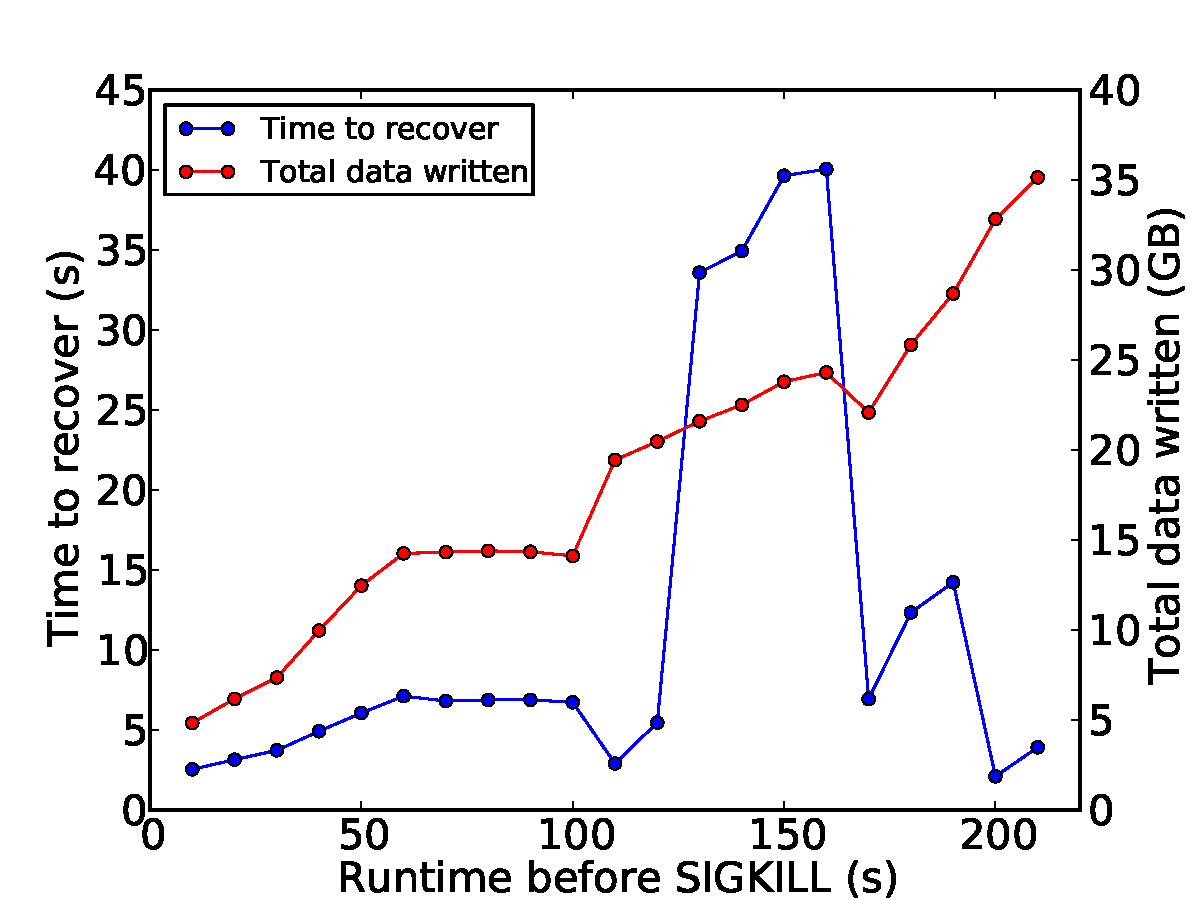
\includegraphics[width=3.5in]{figures/checkpointing.pdf}
   \caption{Recovery time after writing data to LSVD file for a specific amount of time.}
   \label{fig:checkpointing}
\end{figure}

\subsection{File System Benchmarks}

\begin{figure}
  \centering
   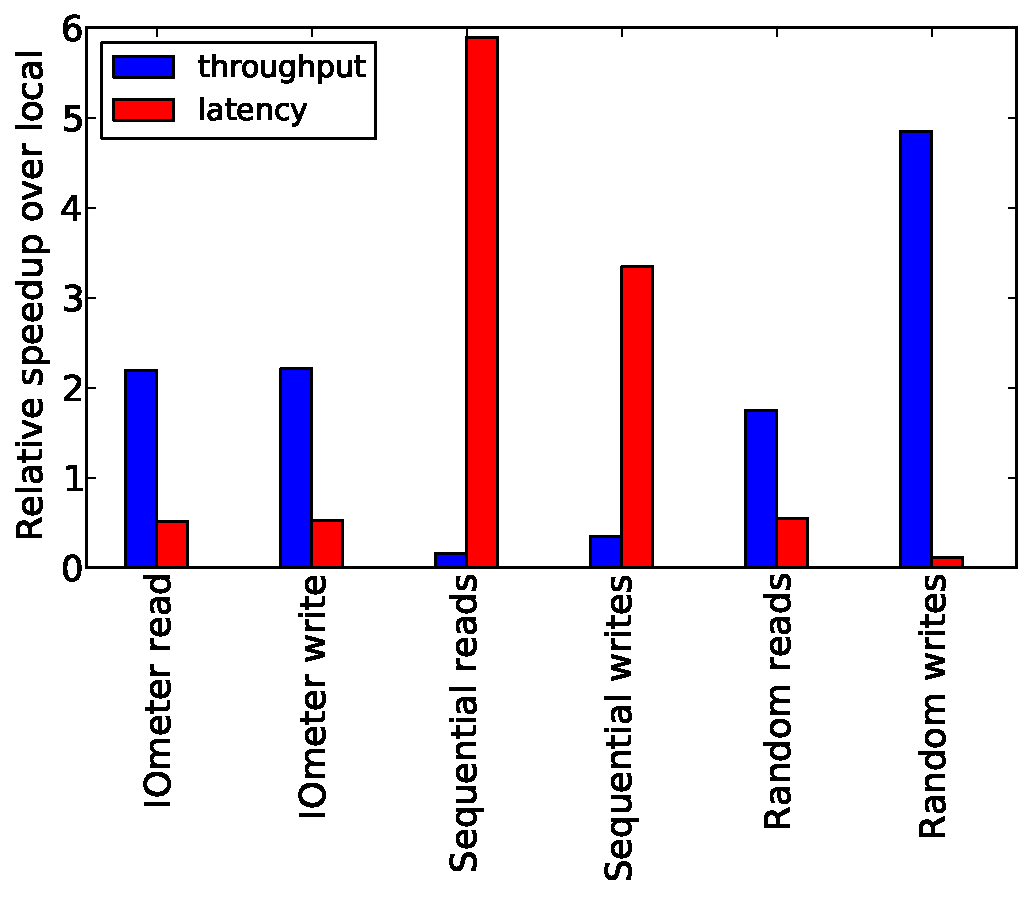
\includegraphics[width=3.5in]{figures/benchmarks.pdf}
   \caption{File system benchmarks \XXX{TODO}}
   \label{fig:checkpointing}
\end{figure}
